\documentclass[11pt]{report}

\special{papersize=8.5in,11in}

\topmargin -0.5in \oddsidemargin 0.00in \evensidemargin 0.00in
\textwidth 6.75in \textheight 9.0in \headheight 0.25in \headsep
0.25in \footskip 0.5in \hoffset 0in \marginparpush 0.0in
\marginparwidth 0.0in \marginparsep 0.2in

\setcounter{page}{1}

\newcommand{\D}{\displaystyle}\newcommand{\T}{\textstyle}
\newcommand{\e}{{\mathrm{exp}}}
\newcommand{\dd}{{\mathrm d}}
\newcommand{\comment}[1]{}
\newcommand{\mb}{\mathbf}
\reversemarginpar

\usepackage[final]{graphicx}
\usepackage{fancyhdr}
%\graphicspath{{Papers/}}
\usepackage{amsthm,amssymb,amsmath}
\usepackage{cite}
\usepackage{geometry}
\usepackage{amsmath}
\usepackage{booktabs}
\usepackage{color}
\usepackage{setspace}
\usepackage{subfigure}
\usepackage{url}
%\usepackage{algorithm}
\usepackage{algorithmic}
\usepackage[ruled]{algorithm2e}
%\usepackage[top=2.5cm, bottom=2.5cm, right=3.5cm, left=3.5cm]{geometry}
\geometry{a4paper,scale=0.8}
\setcounter{secnumdepth}{3}

\title{Research Progress Report}

\author{Botao Zhu}

\begin{document}
	
	\maketitle
	\lhead{\sf Research Progress Report-7th} \chead{} \rhead{\sf Botao Zhu}
	\lfoot{CTRG, University of Saskatchewan} \cfoot{} \rfoot{Page \thepage}
	\renewcommand{\footrulewidth}{1.0pt}
	\renewcommand{\headrulewidth}{2.0pt}
	\renewcommand{\arraystretch}{1.3}
	\pagestyle{fancy}
	
	\renewcommand{\thesection}{\arabic{section}}
	
	\section{Reading and Research Activities}
	
	\subsection{Reading Summary}
	\subsubsection{Energy-efficient modified LEACH protocol for IoT application}
	\begin{itemize}
		\item \textbf{Algorithm description}\\
			\noindent \cite{8465504} extends the application of LEACH to IoT for the first time, which modifies the original LEACH protocol to maintain uniform energy throughout the network.\\ Firstly, it proposes a new LEACH algorithm with hard and soft threshold strategies to select cluster heard (CH) effectively. According to conventional LEACH protocol, a CH is not eligible for selection of CH for the next $1/P$ rounds if it had been the CH. However, in some cases, a CH maybe does not consume much energy in this round and it still can remain CH in the next rounds. This paper solves the above problem by setting a threshold value, which means any CH with more energy than the threshold value can continue to be CH with the same cluster for the next round. In this way, the energy cost in the phase of set-up for a new CH selection can be saved in each round, because there is no need to send information to re-select the CH and notify members to join the cluster. Assuming there are n nodes in a WSN, the energy of CH replacement process can be denoted  by $P_\text{HR}$ during the set-up phase in each round
		\begin{equation}
		P_\text{HR} = \left(P_{k \text{Tx}}P_{\text{Tx}} + P_{k \text{Rx}}P_{\text{Rx}}\left(nC-1\right)\right)RnC
		\end{equation}
		where $C$ is the percentage of clusters, $R$ is the count of CH replacement, $P_{k\text{Tx}}$ and $P_{k\text{Rx}}$ are the transmitted and received packet sizes respectively, $P_{\text{Tx}}$ and $P_{\text{Rx}}$ are the energy cost of transmission and reception of 1 byte data. 
		The total energy of each cluster
		\begin{equation}
		P_{\text{WEC}} = E_{\text{Init}} \times nC
		\end{equation}
		where $P_{\text{WEC}}$ is the initial energy of each node.
		The energy consumption of each cluster 'i' during each round, denoting $N = nC$
		\begin{equation}
		P_{\text{HR}}\left(i\right) = \left(\left(N_i - 1\right)P_{\text{kTx}}P_{\text{kRx}} \times P_{\text{kRx}}P_{\text{Rx}}\right) + \left(\left(N_i-1\right)P_{\text{kRx}}P_{Rx} + \left(N_i-1\right)P_{\text{kTx}}P_{\text{Tx}}\right)
		\end{equation}
		The number of rounds can be calculated by
		\begin{equation}
		\text{Count}_{Rnd} = \frac{P_{HR}}{P_{WEC}} \times 100
		\end{equation}
		So, the minimum level of energy can be estimated by the following equation, which can be considered as the threshold value
		\begin{equation}
		P_{\text{Th}} = \text{Count}_{Rnd}\left(P_{\text{kTx}} + P_{\text{kRx}}\right)P_{\text{Tx}}
		\end{equation}
		
		\noindent Secondly, because the energy requirement of intra-cluster transmission and inter-cluster transmission is different, a CH uses a high energy amplification level. When it becomes a common node in the following rounds, it will choose a low power level. Fig. \ref{fig1} shows the whole algorithm flowchart.
		\begin{figure}[h!]
			\centering
			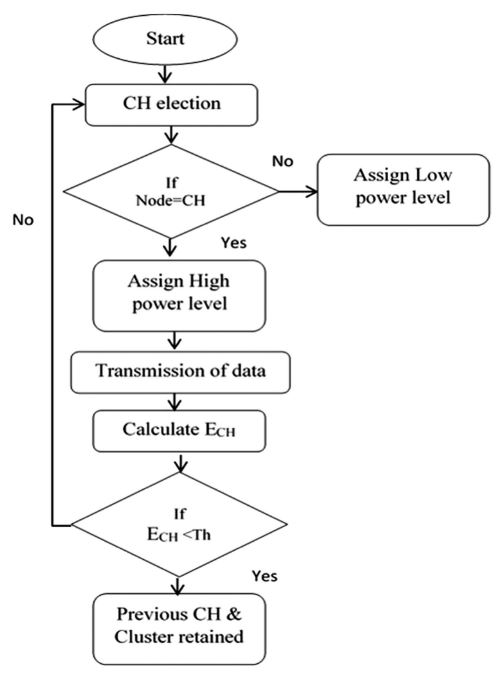
\includegraphics[width=0.5\linewidth]{1th.jpg}
			\caption{IoT LEACH algorithm}
			\label{fig1}
		\end{figure}
	\end{itemize}
    \begin{itemize}
    	\item \textbf{Simulation analysis}
    	\begin{figure}[!h]
    		\subfigure[Average residual energy]{
    			\begin{minipage}[h]{0.5\linewidth}
    				\centering
    				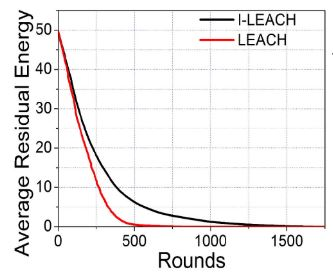
\includegraphics[width=3in]{2sea.jpg}
    				\label{2sea}
    			\end{minipage}
    		}%
    		\subfigure[Throughput]{
    			\begin{minipage}[h]{0.5\linewidth}
    				\centering
    				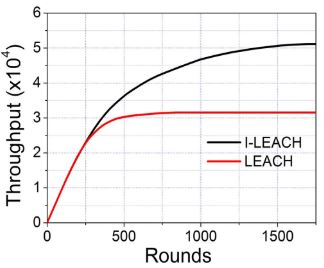
\includegraphics[width=3in]{2seb.jpg}
    				\label{2seb}
    			\end{minipage}
    		}%
    		\centering
    		\caption{Network performance}
    	\end{figure}
    	
    	\noindent Fig. \ref {2sea} shows that the average residual energy of LEACH comes to zero after 500 rounds, however, the average residual energy of IoT LEACH comes to zero after around 1250 rounds. In Fig. \ref {2seb}, the throughput of IoT LEACH is much higher than that of LEACH. After completion of approximately only 750 rounds, the number of active nodes goes completely to 0 for LEACH, whereas with IoT LEACH, some nodes are still alive till 1500 rounds, shown in Fig. \ref{3rd}.
    	\begin{figure}[!h]
    		\subfigure[Dead nodes]{
    			\begin{minipage}[h]{0.5\linewidth}
    				\centering
    				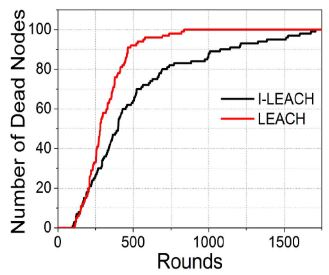
\includegraphics[width=3in]{3rda.jpg}
    				\label{3rda}
    			\end{minipage}
    		}%
    		\subfigure[Alive nodes]{
    			\begin{minipage}[h]{0.5\linewidth}
    				\centering
    				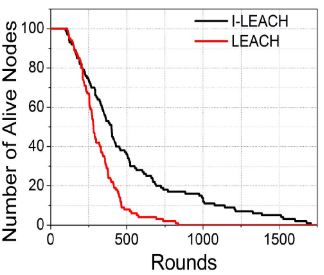
\includegraphics[width=3in]{3rdb.jpg}
    				\label{3rdb}
    			\end{minipage}
    		}%
    		\centering
    		\caption{Lifetime metrics}
    		\label{3rd}
    	\end{figure}
    \end{itemize}

    \newpage
    \subsubsection{Energy efficient clustering protocol based on kmeans-midpoint algorithm for enhanced network lifetime in wireless sensor network}
    \begin{itemize}
    	\item \textbf{Algorithm description}\\
    	\noindent \cite{7763028} considers residual energy as the parameter in addition to euclidean distance used in basic K-means algorithm for approximate CH selection. It mainly has three contributions:\\
    	1. It gives the optimum number of desired clusters based on the size of region and the number of nodes.
    	\begin{equation}
    	k_{opt} = \frac{\sqrt{N}}{\sqrt{2 \pi}} \sqrt{\frac{\varepsilon_{fs}}{\varepsilon_{mp}}} \frac{M}{d^2_{BS}}
    	\end{equation}
    	where $M$ is the length and width of region, N is the total number of nodes, $d_{BS}$ is the distance from CH to BS, $\varepsilon_{fs}$ is the parameter for free model and $\varepsilon_{mp}$ is the parameter for multipath model. \\
    	2. For CHs selection, midpoint method is used in order to balance the number of cluster and the load of CHs, which prolongs the network lifetime. \\
    	
    	\begin{algorithm}[H]
    		\caption{Midpoint algorithm for initial CH selection}
    		\LinesNumbered
    		\KwIn{\\
    			$D$ = set of $n$ data points \\
    			$k_{opt}$ = optimum number of desired clusters }
    		\KwOut{\\
    			$k_{opt}$ number of initial centroids}
    		\begin{algorithmic}[1]
    			\STATE Compare the distance from origin for each data point
    			\STATE Sort the distance obtained in step 1, sort the data points in accordance with the distance
    			\STATE Partition the sorted data points into $k_{opt}$ equal sets
    			\STATE In each set, take the middle point as the initial centroid
    		\end{algorithmic}
    	\end{algorithm}
    	\noindent 3. The residual energy of node is considered as the parameter of CH selection in addition to the euclidean distance used in basic kmeans. To maintain the connectivity of the network, residual energy of the CH is checked every round. If the node's residual energy is less than the threshold value, it cannot be selected as CH. The threshold energy is given by
    	\begin{equation}
    	E_{threshold} = lE_{elec}\left(\frac{N}{k_{opt}}-1\right) + lE_{DA}\frac{N}{k_{opt}} + lE_{elec} + l\varepsilon_{fs}d^2_{toBS}
    	\end{equation}
    	
    	\noindent The proposed algorithm has three phases:\\
    	\noindent Phase 1: initial CH selection, shown in algorithm 1.\\
    	\noindent Phase 2: balanced cluster formation.\\
    	\begin{algorithm}[H]
    		\caption{Balanced cluster formation}
    		\LinesNumbered
    		\KwIn{\\
    			$D$ = set of $n$ data points \\
    			$k_{opt}$ = optimum number of desired clusters\\
    			$E_{threshold}$ = threshold energy }
    		\KwOut{\\
    			$k_{opt}$ A set of $k_{opt}$ clusters}		
    		\begin{algorithmic}[1]
    			\STATE Apply midpoint method in algorithm 1 to choose $k_{opt}$ out of $D$ sensor nodes as initial cluster heads;
    			\STATE Repeat
    			\STATE Each of the remanining nodes decides to join its nearest CH according to the euclidean distance;
    			\STATE Centroid of each cluster is calculated as
    			\begin{equation*}
    			Centroid \left(X,Y\right) = \left(\frac{1}{s} \sum_{i=1}^{s}x_i, \frac{1}{s} \sum_{i=1}^{s}y_i\right)
    			\end{equation*}
    			\STATE After cluster formation, based on the distance from the centroid, and ID number is allotted to each node of a cluster, assigning smaller number to the closer one
    			\STATE \For{all selected cluster heads}{
    				\eIf{Residual energy of cluster head>$E_{threshold}$}{The node will remain as cluster head}{Check ID number of all nodes in that cluster. \\
    					The node in the next order of ID number is selected as a new CH}}
    			\STATE The newly selected CHs inform other nodes about the CHs change.
    			\STATE Until the cluster heads are not changed any more.
    		\end{algorithmic}
    	\end{algorithm}
    	\noindent Phase 3: Data communication. \\
    	\begin{algorithm}[H]
    		\caption{Data communication}
    		\LinesNumbered
    		\KwIn{\\
    			$D$ = set of $n$ data points \\
    			$\left(CH_1, CH_2,...,CH_{k_{opt}}\right)=$ a set of $k_{opt}$ clusters\\
    			$d_{threshold}$ = threshold distance}	
    		\begin{algorithmic}[1]
    			\STATE Nodes send data packet to their CHs.
    			\STATE Calculate the distance  between each elected CH and BS$(d_{BS})$.
    			\STATE \eIf{$d_{BS}<d_{threshold}$}{
    				Cluster head directly commuication to the BS}{It selects the nearest neighbour cluster head whose $d_{BS}$ is less than $d_{threshold}$ to communicate to the BS.}
    			
    		\end{algorithmic}
    	\end{algorithm}
    \end{itemize}
	\begin{itemize}
		\item \textbf{Simulation analysis}\\
		Fig.\ref {4tha} shows uneven number of nodes by using basic kmeans, CH of the heavily loaded cluster with 39 nodes will be exhausted much earlier than the other clusters. After applying the proposed approach, a particular cluster contains maximum 29 nodes and minimum 21 nodes, which is much closer to the average number of nodes. \\
		\begin{figure}[!h]
			\subfigure[Using basic kmeans approach]{
				\begin{minipage}[h]{0.5\linewidth}
					\centering
					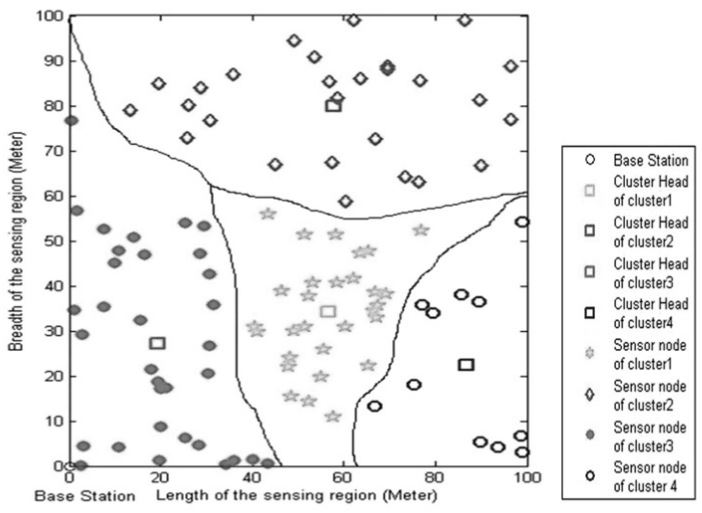
\includegraphics[width=3in]{4tha.jpg}
					\label{4tha}
				\end{minipage}
			}%
			\subfigure[Using proposed approach]{
				\begin{minipage}[h]{0.5\linewidth}
					\centering
					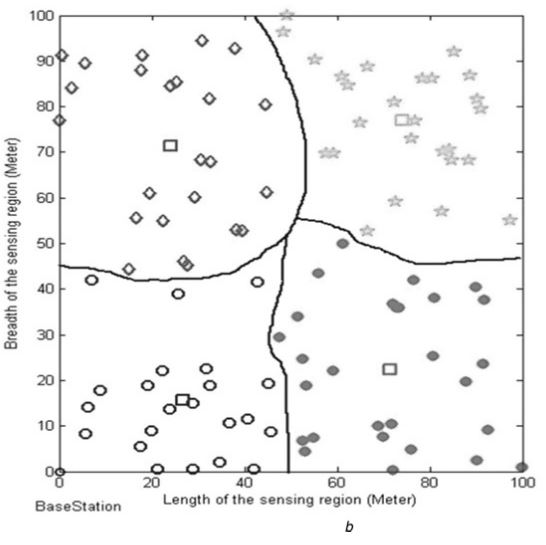
\includegraphics[width=2.5in]{4thb.jpg}
					\label{4thb}
				\end{minipage}
			}%
			\centering
			\caption{Lifetime metrics}
			\label{4th}
		\end{figure}
		The number of nodes which are alive using LEACH-B, BPK-means, basic Kmeans, Mk-means and the proposed protocol are compared with respect to the number of rounds as shown in Fig. \ref {fig5}. It clearly shows that proposed protocol provides better network lifetime compared to the above mentioned algorithms and helps to provide enhanced network lifetime to a great extent. \\
		\begin{figure}[h!]
			\centering
			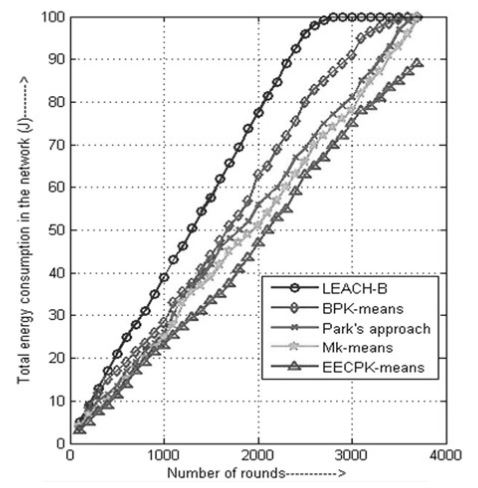
\includegraphics[width=0.5\linewidth]{5th.jpg}
			\caption{Number of alive nodes with respect to number of rounds}
			\label{fig5}
		\end{figure}
	    In Fig. \ref {fig6}, it shows the comparison of the energy consumption of the proposed protocol with LEACH-B, BPK-means, basic Kmeans and Mk-means algorithm with respect to the number of rounds. It shows that the proposed protocol can reduce energy consumption significantly compared to above mentioned algorithms.
	    \begin{figure}[h!]
	    	\centering
	    	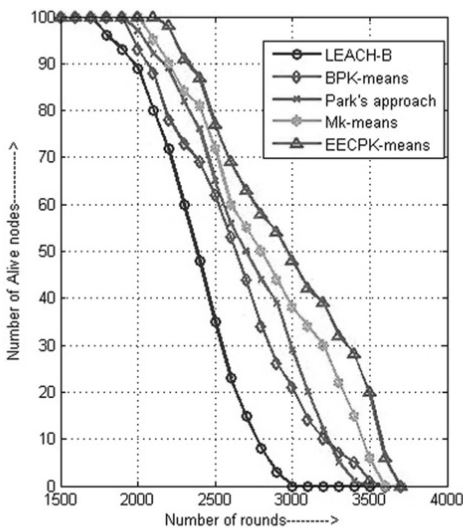
\includegraphics[width=0.5\linewidth]{6th.jpg}
	    	\caption{Energy consumption with respect number of rounds}
	    	\label{fig6}
	    \end{figure}
	\end{itemize}
	\subsubsection{EEM-LEACH: Energy efficient multi-hop LEACH routing protocol for clustered WSNs}
	
	\cite{6993070} presents a cluster based multi-hop routing protocol EEM-LEACH characterized by \\
	1. Cluster head selection based on residual energy and average energy consumption of nodes.\\
	2. Multi-hop inter cluster communication that choose a choose a multi-hop path with minimum communication cost from each node to the base station. \\
	3. Direct communication by nodes near to the base station. 
	\begin{itemize}
		\item \textbf{Algorithm description}\\
		At the beginning of set-up phase, each node chooses a random number of 0 and 1, every node computes the threshold $T(n)$ as follows:\\
		\begin{equation}
		T(n) = \left\{ \begin{array}{ll}
		\frac{p}{1-p \times \left(r mod 1/p\right)}\times P\left(RE\right), n \in G\\
		0         \,                      ,otherwise
		\end{array} \right.
		\end{equation}
		\begin{equation}
		P(RE) = \left\{ \begin{array}{ll}
		\frac{E_{res}-E_{avg}}{E_{res}},if \, E_{res} > E_{avg}\\
		1-E_{avg}, otherwise 
		\end{array} \right.
		\end{equation}
		where $p$ is the desired percentage of cluster heads, $r$ is the current round, $G$ is the set of nodes that have not become the cluster head in last $1/p$ rounds, $E_{res}$ is the residual energy. If the chosen random number $< T(n)$, then n becomes the cluster head for the current round $r$. \\
		Once cluster heads are selected, base station at the center sends CHADV message to its neighbor. CHADV message contains a communication cost field that consists of cost metric of the base station/cluster head that has sent the message. Initially, cost metric is zero at the base station and large value at each cluster head. When a cluster head $v$ receives CHADV messages from base station/cluster head $u$, communication cost metric $c$ is computed as follows:
		\begin{equation}
		c = \left\{ \begin{array}{ll}
		C(u) + d^2_{uv}, d_{uv} > d_0\\
		C(u) + d^2_{uv}, d_{uv} < d_0
		\end{array} \right.
		\end{equation}
		where $C(u)$ is the cost metric at $u$ and $d_{uv}$ is the distance between $u$ and $v$. The cost metric at $v$ is
		\begin{equation}
		C(v) = min(C(v),c)
		\end{equation}
		Each cluster head $v$ receives CHADV message from multiple cluster heads/base station, computes cost metric for each and choose the minimum cost metric $c'$ after $t'$ time from the receipt of first CHADV message where $t'$ is the propagation delay for the first CHADV message received. If cost metric $c'$ is computed when cluster head $v$ received CHADV message from $u$, then $u$ is selected as the next hop of $v$ in the multi-hop path to the base station. Also, CHADV message with communication cost field updated as $C(v)=c'$ is sent to $v's$ neighbors. If a cluster head receives at least one CHADV message after sending the first CHADV message, cost metric is computed. If the cluster head's cost metric is updated, then a CHADV message is sent with updated communication cost field. Thus, by propagating cost via CHADV message, multi-hop path with minimum communication cost from each cluster head to base station is determined.
		The set-up phase is shown in Fig. \ref {fig7}. 
		\begin{figure}[h!]
			\centering
			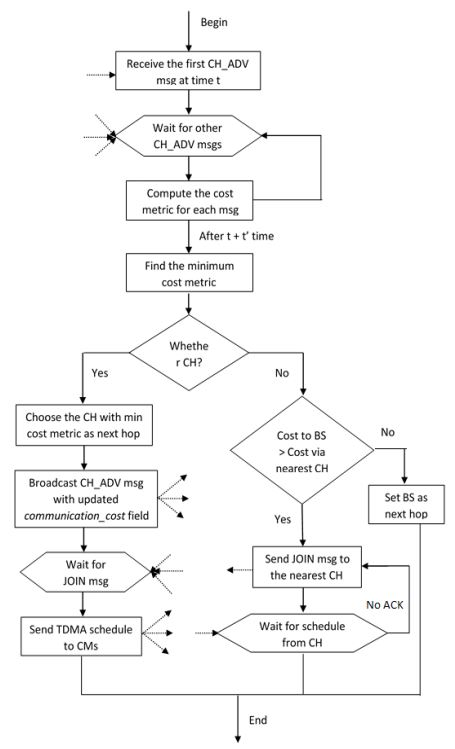
\includegraphics[width=0.45\linewidth]{7th.jpg}
			\caption{Set-up phase of EEM-LEACH}
			\label{fig7}
		\end{figure}
		During the steady state phase, once cluster members receive BEGIN message from the cluster head, each member node sends data in the allotted time slot, shown in Fig. \ref {fig8}. 
		\begin{figure}[h!]
			\centering
			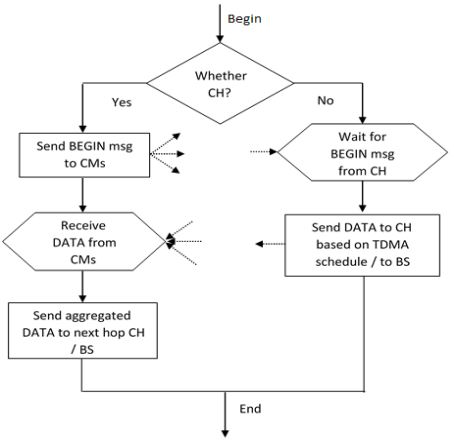
\includegraphics[width=0.45\linewidth]{8th.jpg}
			\caption{Steady state phase of EEM-LEACH}
			\label{fig8}
		\end{figure}
	\end{itemize}
	\begin{itemize}
		\item \textbf{Simulation analysis}\\
		Fig.\ref{fig9} shows that the proposed EEM-LEACH protocol has improved lifetime than existing protocols. For a smaller network with area 100m $\times$ 100m, until the first node's death, EEM-LEACH has $42\%$ and $41\%$ better lifetime than LEACH and M-LEACH respectively.\\   
		\begin{figure}[h!]
			\centering
			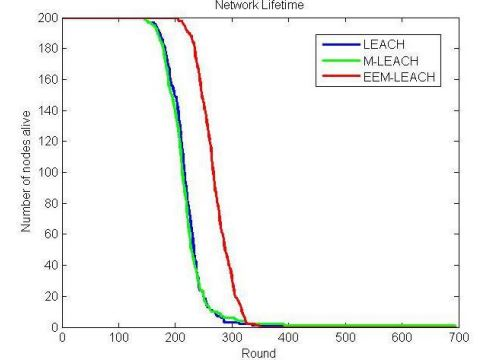
\includegraphics[width=0.45\linewidth]{9th.jpg}
			\caption{Network lifetime for 100m $\times$ 100m size network}
			\label{fig9}
		\end{figure}
	
		\noindent The proposed EEM-LEACH protocol has less energy consumption than LEACH and M-LEACH because of choosing a multi-hop path with minimum communication cost, shown in Fig.\ref{fig10}.\\
		\begin{figure}[h!]
			\centering
			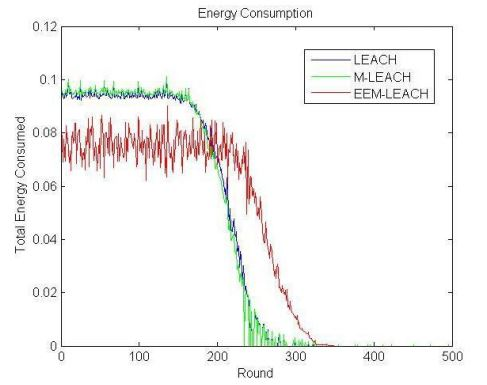
\includegraphics[width=0.45\linewidth]{10th.jpg}
			\caption{Energy consumption for 100m $\times$ 100m size network}
			\label{fig10} 
		\end{figure}
	
		\noindent Fig. \ref{fig11} shows data packet delivery is better for proposed protocol than LEACH and M-LEACH.
		\begin{figure}[h!]
			\centering
			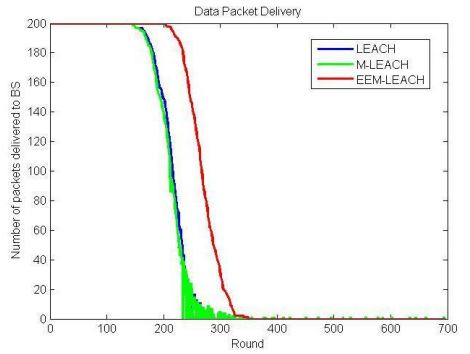
\includegraphics[width=0.45\linewidth]{11th.jpg}
			\caption{Data packet delivery for 100m $\times$ 100m size network}
			\label{fig11} 
		\end{figure}
	\end{itemize}
	
	\subsubsection{Other papers}
	\cite{article} has presented the LEACH-SAGA routing protocol that is based on optimization techniques of simulated annealing and genetic algorithms for better energy distribution among the sensor nodes in the WSN. The LEACH-SAGA routing protocol is a completely centralized control algorithm which is executed at the BS. Initially it forms optimal numbers of clusters accomplished by simulated annealing and genetic algorithms. After the formation of clusters, the BS calculates the centroid of each cluster. In the selection of the CH, the BS considers the residual energy of the sensor nodes and the distance of the sensor node from the centroid. The sensor nodes with energy greater than the average energy of the cluster become the set of possible CHs in each cluster. The BS selects the final CHs from the possible CHs set based on the minimum distance from the centroid. In the steady state phase, member nodes of the clusters communicate with their respective CHs and CHs then transmit the aggregated data to the BS via other CHs. The LEACH-SAGA routing protocol outperforms LEACH in terms of network lifetime. It also claims even distribution of the CH in the network with less energy consumption. The main issues with this protocol are scalability, delay and complexity.\\
	
	\noindent \cite{Liu2011LEACHGAGA} proposes a genetic algorithm (GA) based adaptive clustering protocol with an optimal probability for cluster formation and selection. Initially, all nodes participate in the candidate CH (CCH) selection process by generating a random number $r$ and comparing this $r$ with threshold $T(s)$. If the value of $r$ is less than $T(s)$, based on a probability value $p_{sat}$, then the node is selected as CCH. After the selection of initial CCH, all nodes send their status messages containing their id, location information and CCD information. Based on this information, the BS finds the optimal probability $P_{opt}$ for formation of optimal clusters $K_{opt}$ with the help of GA. The GA searches the solution space to determine the $P_{opt}$ using an evolutionary optimization process including probabilistic transitions and non-deterministic rules with crossover and mutation operators. After selecting $P_{opt}$, the BS broadcasts the value of $P_{opt}$ to all sensor nodes n. The set up and steady state phase are the same as in LEACH.
	The performance of this protocol is compared in two scenarios based on the BS position. In the first case, the BS is located in the centre of the network and in the second case, it is situated outside of the network. In both cases, LEACH-GA performs better than LEACH in
	terms of energy efficiency but it suffers from message overhead and scalability.
	
	
	\subsection{Course}
	Finished the chapter 1 of Structuring Machine Learning Projects, Coursera, https://www.deeplearning.ai/deep-learning-specialization/
	
	\section{Objectives for the Next 2 Weeks}
	\subsection{Reading} 
	By reading the papers, it is found that the most important parts of LEACH and improved LEACH protocols are the selection of cluster heads and the formation of the clusters. Some papers have studied to solve above problems by Kmeans. For the next two weeks, I will continue reading papers that use Kmeans in LEACH and try to propose an improved Kmeans LEACH protocol. 
	
	\section{Advisor's Comments}
	
	\bibliographystyle{IEEEtran}
	\bibliography{janbib}
	
\end{document}